%!TEX root = ../thesis.tex

\chapter{Grundlagen}
\label{chap:fundamentals}
\todo{Grundlagen einteilen und schreiben}

\section{Darts}
Grundregeln von Darts erklären.
Grundsätzliche Darts Regeln erklären
\section{Aufbau der Testumgebung}

\section{Grundlagen Bildverarbeitung}
\label{sec:basics}
Das Pinhole Camera Modell sieht wie folgt aus: \autocite{Zhang2000}.
\begin{figure}
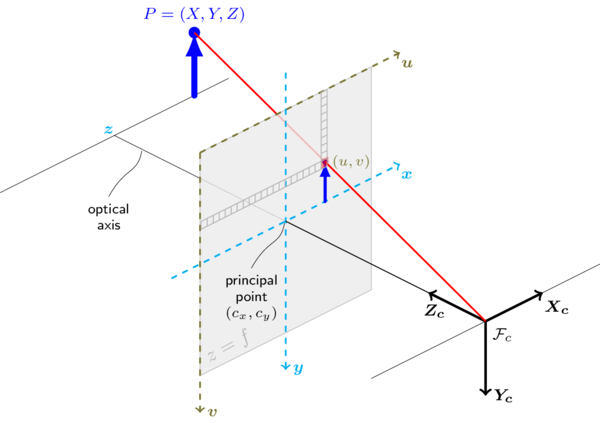
\includegraphics[scale =0.75]{media/pinhole_camera_model}\\
\caption{\textbf{Pinhole Camera Modell von.\autocite{OpencvCamera2016}}
}
\label{Fig:pinhole}
\end{figure}
\vspace{11mm}
	
	\vspace{3mm}

\todo{pinhole Camera Modell erläutern}
\todo{opencv Benutzung erklären}
OpenCV ist eine \autocite[512--]{Medioni:2004:ETC:993884}

